\documentclass[12pt,a4paper]{article}
\usepackage{amsmath,amssymb,makecell,fancyhdr,enumerate,arcs,physics,tasks,mathrsfs,graphics}
\usepackage{tikz,tikz-3dplot,tkz-euclide,tkz-tab,tabvar,pgfplots,esvect}
\usepackage[top=1.5cm, bottom=1.5cm, left=2cm, right=1.5cm]{geometry} 
\usepackage[hidelinks,unicode]{hyperref}
\usepackage[utf8]{vietnam}
\usepackage[solcolor]{ex_test}
\usetikzlibrary{shapes.geometric,shadings,calc,snakes,patterns,arrows,intersections,angles,backgrounds,quotes}
\usepgfplotslibrary{fillbetween}
\pgfplotsset{compat=newest}
\tikzset{point style/.append style={color=white}}
\def\vec{\overrightarrow}
\newcommand{\hoac}[1]{\left[\begin{aligned}#1\end{aligned}\right.}
\newcommand{\heva}[1]{\left\{\begin{aligned}#1\end{aligned}\right.}
\newcommand{\hetde}{\centerline{\rule[0.5ex]{2cm}{1pt} HẾT \rule[0.5ex]{2cm}{1pt}}}
\newcommand{\tentruong}{THPT Nguyễn Hữu Cảnh}
    \newcommand{\tengv}{GV Nguyễn Văn Sang}
    \newcommand{\tenkythi}{Bộ Đề Ôn Thi HKII}
    \newcommand{\tenmonthi}{Môn: Toán - Đề Số 2}
    \newcommand{\thoigian}{90}
    \newcommand{\tieude}[3]{
	\noindent
	%Trái
	\begin{minipage}[b]{7cm}
		\centerline{\textbf{\fontsize{13}{0}\selectfont \tentruong}}
		\centerline{\textbf{\fontsize{13}{0}\selectfont \tengv}}
		\centerline{(\textit{Đề thi có #1\ trang})}
		\centerline{\textit{ }}
	\end{minipage}\hspace{1.5cm}
	%Phải
	\begin{minipage}[b]{9cm}
		\centerline{\textbf{\fontsize{13}{0}\selectfont \tenkythi}}
		\centerline{\textbf{\fontsize{13}{0}\selectfont \tenmonthi}}
		\centerline{\textit{\fontsize{12}{0}\selectfont Thời gian làm bài \thoigian \ phút }}
		\centerline{\textit{\fontsize{12}{0}\selectfont (Đề có 13 câu trắc nghiệm, 4 câu đúng sai, 6 câu điền đáp án)}}
	\end{minipage}
	\begin{minipage}[b]{13cm}
		\vspace*{.75cm}
		\textbf{Họ và tên thí sinh: }{\tiny\dotfill}\\
		\textbf{Số Báo Danh: }{\tiny\dotfill}
	\end{minipage}
	\begin{minipage}[b]{8cm}
		\hspace*{1cm}\fbox{\bf Mã đề thi #3}
	\end{minipage}
}
\newcommand{\chantrang}[2]{\rfoot{Trang \thepage/#1 $-$ Mã đề #2}}
\pagestyle{fancy}
\fancyhf{}
\renewcommand{\headrulewidth}{0pt}
\def\colorEX{}% màu phương án đúng
\renewtheorem{ex}{\color{blue!80!black}\textbf{Câu}}
    
    \newcommand{\made}{467}
    \begin{document}   
    \tieude{\pageref{\made}}{0}{\made}
    \chantrang{\pageref{\made}}{\made}
     \begin{center}
	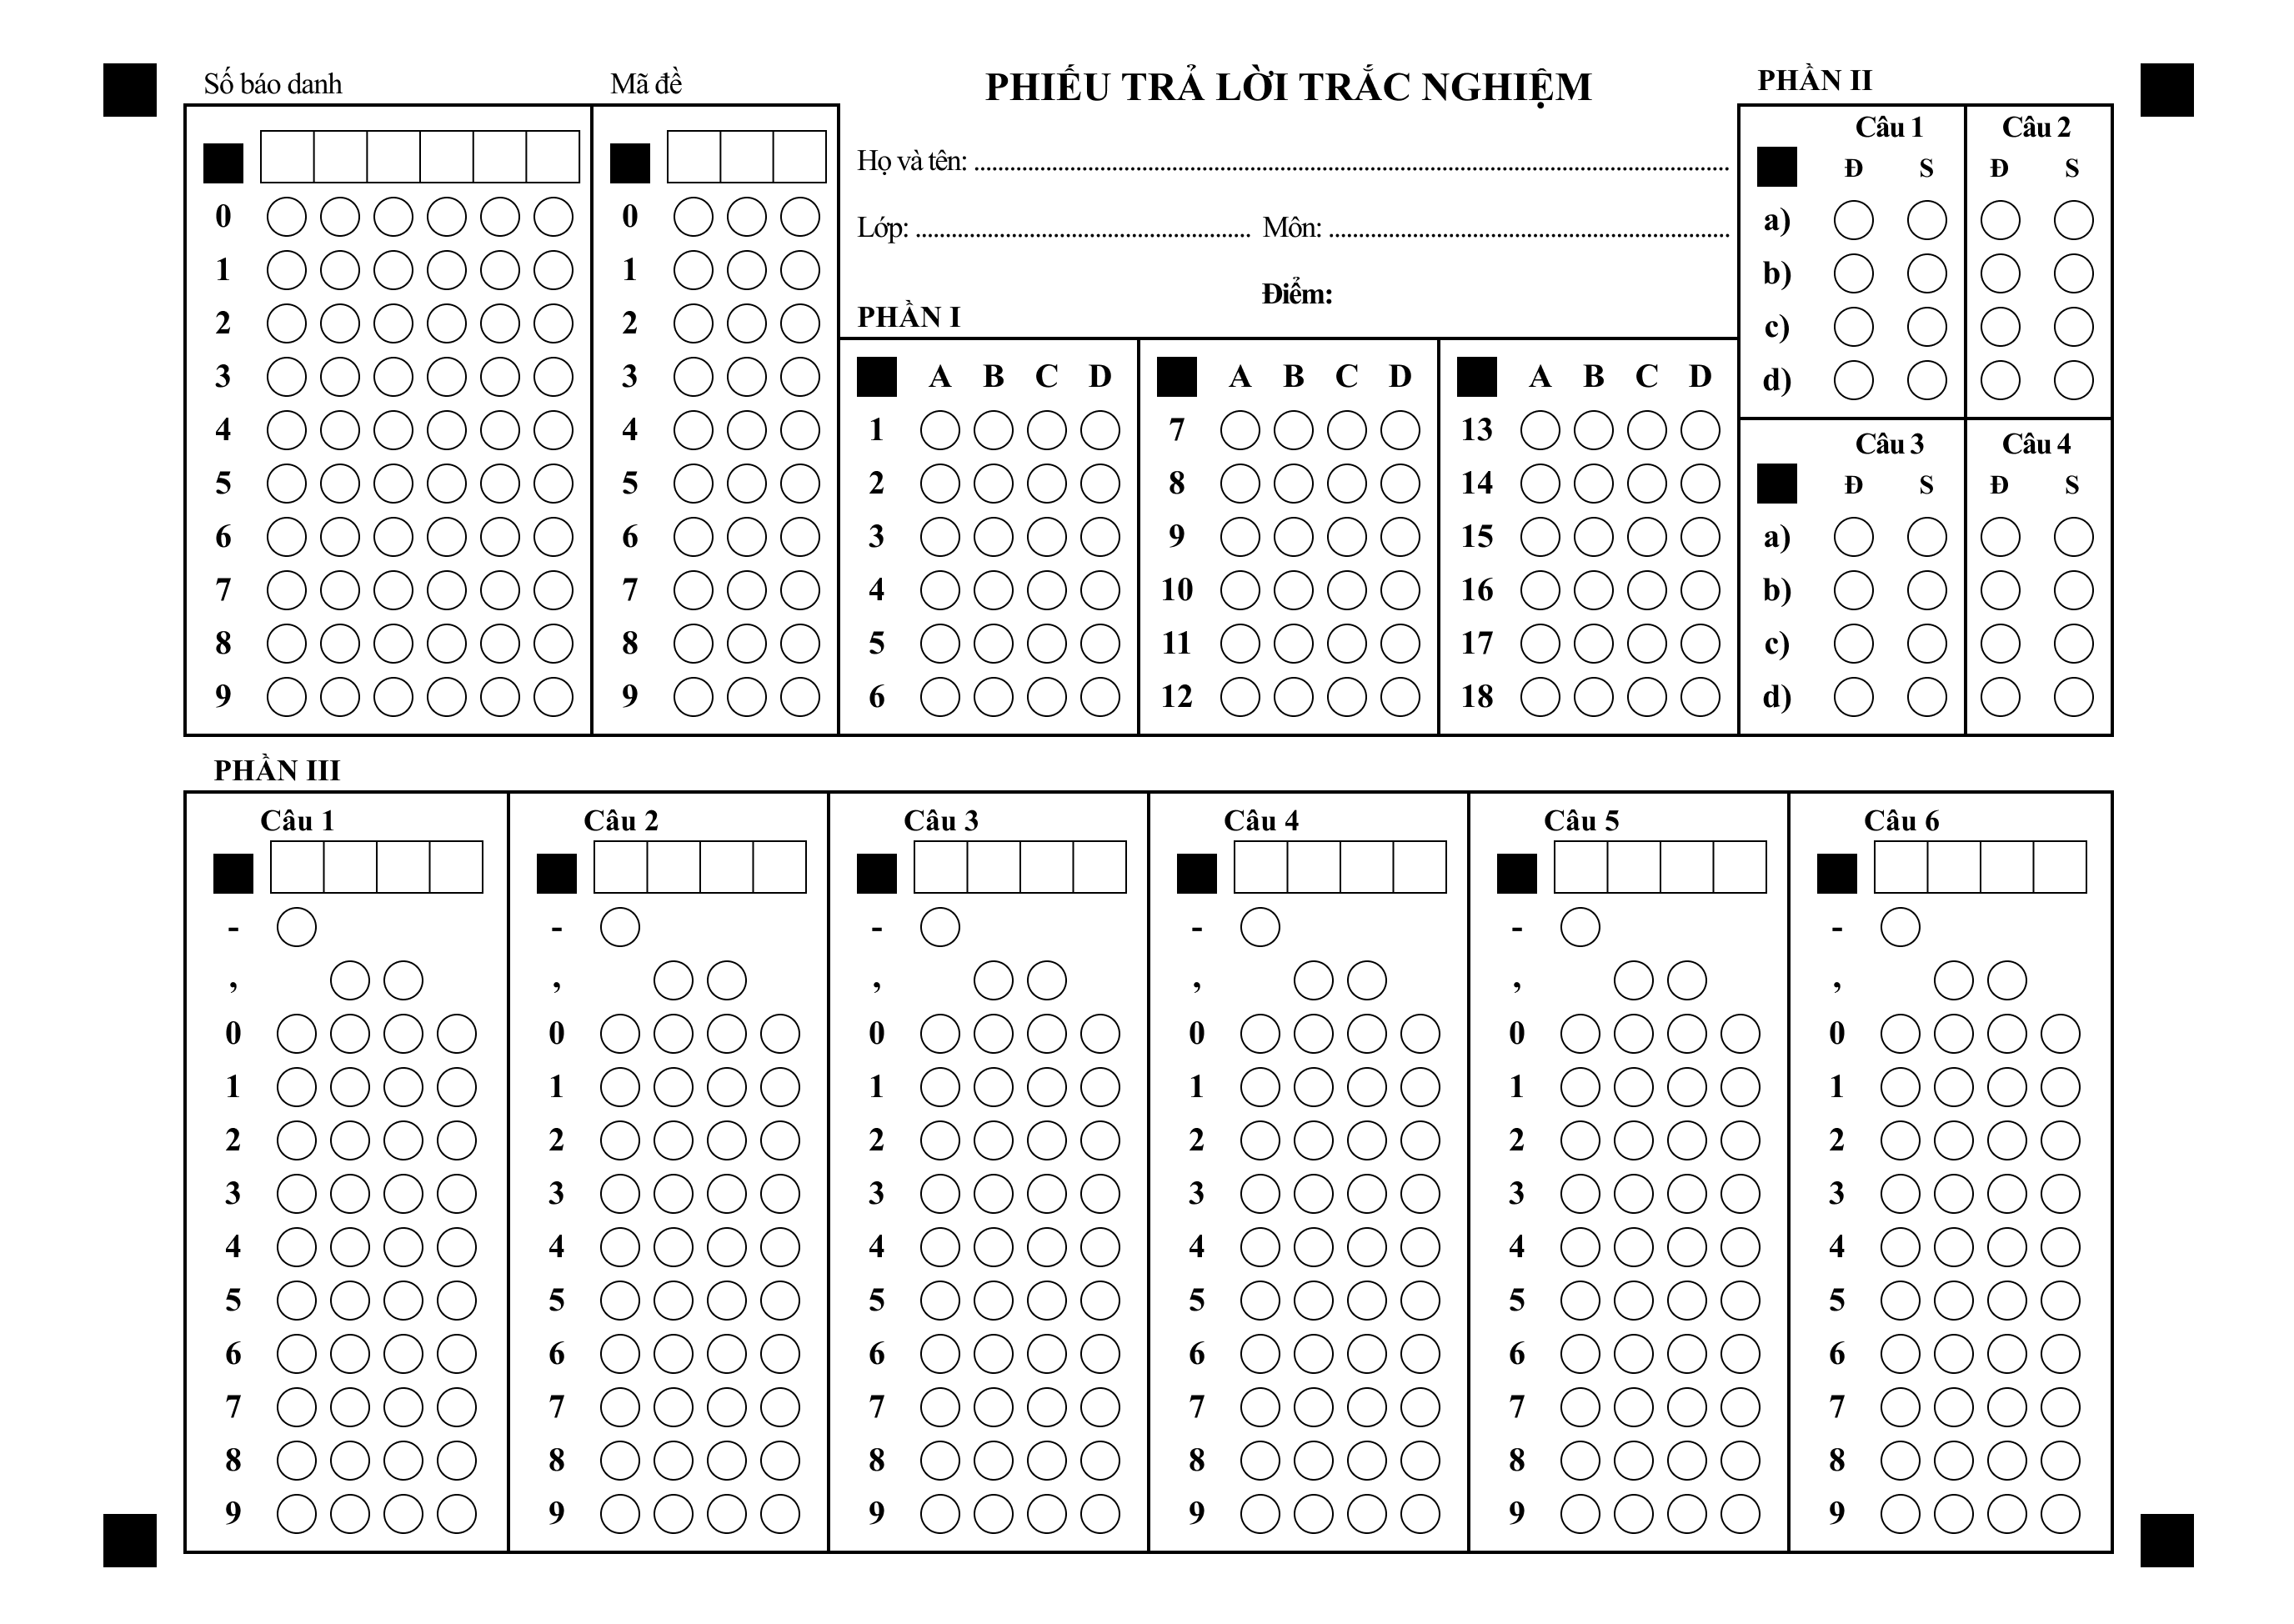
\includegraphics[width=1\textwidth]{UnT18.4.6.png}
\end{center}
    \subsection*{PHẦN I. Câu trắc nghiệm nhiều phương án lựa chọn. Thí sinh trả lời từ câu 1 đến câu 13. Mỗi câu hỏi thí sinh chỉ chọn một phương án.}
    \setcounter{ex}{0}
    \Opensolutionfile{ans}[ans-phanI]
\begin{ex}%[2D4N2-1]
	Cho $\displaystyle\int\limits_2^5 f\left( x \right)\mathrm{d}x=10$. Kết quả $\displaystyle\int\limits_5^2 \left[ 2-4f\left( x \right) \right]\mathrm{d}x$ bằng
	\choice
{$40$}
{\True $34$}
{$32$}
{$36$}
	\loigiai{
		Ta có
		\allowdisplaybreaks
		\begin{eqnarray*}
			\displaystyle\int\limits_5^2 \left[ 2-4f\left( x \right) \right]\mathrm{d}x &=& 2\displaystyle\int\limits_5^2 \mathrm{d}x-4\displaystyle\int\limits_5^2 f\left( x \right)\mathrm{d}x\\
			&=& -2x \Big|_2^5+4\displaystyle\int\limits_2^5 f\left( x \right)\mathrm{d}x\\
			&=& -2\cdot\left( 5-2 \right)+4\cdot 10=34.
		\end{eqnarray*}
	}
\end{ex}
\begin{ex}%[2H5N2-2]
	Trong không gian $Oxyz$, cho đường thẳng $d\colon \dfrac{x-2}{1}=\dfrac{y-1}{2}=\dfrac{z+1}{2}$ nhận véc-tơ $\overrightarrow{u}=(a;2;b)$ làm véc-tơ chỉ phương. Khi đó $a+b$ bằng
	\choice
{$-5$}
{\True $3$}
{$-3$}
{$5$}
	\loigiai{
		Đường thẳng $d$ có một véc-tơ chỉ phương là $\overrightarrow{u}_d=(1;2;2) \Rightarrow \heva{&a=1\\ &b=2} \Rightarrow a+b=3$.
	}
\end{ex}
\begin{ex}%[2H5H2-7]
	Trong không gian $Oxyz$, cho hai đường thẳng $d_1 \colon \dfrac{x-1}{2}=\dfrac{y+2}{-1}=\dfrac{z-4}{2}$ và \\ $d_2\colon \heva{&x=3+t \\& y=-t \\& z=4}$. Tính góc giữa $d_1$ và $d_2$.
	\choice
{$90^\circ$}
{\True $45^\circ$}
{$30^\circ$}
{$60^\circ$}
	\loigiai{
		Gọi $\varphi$ là góc giữa đường thẳng $d_1$ và $d_2$.\\
		Đường thẳng $d_1$ có véc-tơ chỉ phương $\vec{a}_1=(2;-1;2).$\\
		Đường thẳng $d_2$ có véc-tơ chỉ phương $\vec{a}_2=(1;-1;0).$\\
		Ta có $\cos \varphi=\dfrac{\left| \overrightarrow{a}_{d_1}\cdot\overrightarrow{a}_{d_2} \right|}{\left| \overrightarrow{a}_{d_1} \right|\cdot\left| \overrightarrow{a}_{d_2} \right|}=\dfrac{3}{3\sqrt{2}} \Rightarrow \varphi = 45^\circ$.
	}
\end{ex}
\begin{ex}%[2H5H2-7]
	Trong không gian với hệ tọa độ $Oxyz$, cho mặt phẳng $(\alpha)\colon x-y+2z+1=0$ và đường thẳng $\Delta\colon \dfrac{x}{1}=\dfrac{y}{2}=\dfrac{z-1}{-1}$. Góc giữa $\Delta$ và $(\alpha)$ bằng
	\choice
{$60^\circ$}
{\True $30^\circ$}
{$120^\circ$}
{$45^\circ$}
	\loigiai{ 
		Mặt phẳng $(\alpha)$ có véc-tơ pháp tuyến $\vec{n}_{\alpha}=(1;-1;2)$.\\
		Đường thẳng $\Delta$ có véc-tơ chỉ phương $\vec{u}_\Delta=(1;2;-1)$.\\
		Gọi $\varphi$ là góc giữa đường thẳng $\Delta$ và mặt phẳng $(\alpha)$.\\
		Ta có $\sin\varphi=\dfrac{|1-2-2|}{\sqrt{6}\cdot \sqrt{6}}=\dfrac{1}{2}\Rightarrow\varphi=30^\circ.$
	}
\end{ex}
\begin{ex}%[2H5H3-3]
	Trong không gian $O x y z$, phương trình nào dưới đây là phương trình mặt cầu tâm $I(1 ; 0 ;-2)$, bán kính $r=4$?
	\choice
{$(x-1)^{2}+y^{2}+(z+2)^{2}=4$}
{$(x+1)^{2}+y^{2}+(z-2)^{2}=16$}
{\True $(x-1)^{2}+y^{2}+(z+2)^{2}=16$}
{$(x+1)^{2}+y^{2}+(z-2)^{2}=4$}
	\loigiai{
		Phương trình mặt cầu là $(x-1)^{2}+y^{2}+(z+2)^{2}=16$.
	}
\end{ex}
\begin{ex}%[2H5H3-3]
	Trong không gian $O x y z$, mặt cầu $(S)$ có tâm có tâm $I(1 ;-3 ; 2)$ và đi qua điểm $A(5 ;-1 ; 4)$ là
	\choice
{$(x-1)^{2}+(y+3)^{2}+(z-2)^{2}=\sqrt{24}$}
{\True $(x-1)^{2}+(y+3)^{2}+(z-2)^{2}=24$}
{$(x+1)^{2}+(y-3)^{2}+(z+2)^{2}=\sqrt{24}$}
{$(x+1)^{2}+(y-3)^{2}+(z+2)^{2}=24$}
	\loigiai{
		Mặt cầu có bán kính $R=IA=\sqrt{(5-1)^2+(-1+3)^2+(4-2)^2}=2\sqrt{6}$.\\
		Phương trình mặt cầu là $(x-1)^{2}+(y+3)^{2}+(z-2)^{2}=24$.
	}
\end{ex}
\begin{ex}%[2H5H3-3]
	Trong không gian $O x y z$, cho mặt cầu $(S)$ có tâm $I(-1 ; 4 ; 2)$ và thể tích bằng $\dfrac{256 \pi}{3}$. Phương trình của $(S)$ là
	\choice
{\True $(x+1)^{2}+(y-4)^{2}+(z-2)^{2}=16$}
{$(x-1)^{2}+(y+4)^{2}+(z+2)^{2}=4$}
{$(x-1)^{2}+(y+4)^{2}+(z+2)^{2}=4$}
{$(x+1)^{2}+(y-4)^{2}+(z-2)^{2}=4$}
	\loigiai{
		Mặt cầu có  thể tích bằng $\dfrac{256 \pi}{3}$ nên $\dfrac{4 \pi R^3}{3}=\dfrac{256 \pi}{3} \Leftrightarrow R^3=64 \Leftrightarrow R=4$.\\
		Phương trình mặt cầu là $(x+1)^{2}+(y-4)^{2}+(z-2)^{2}=16$.
	}
\end{ex}
\begin{ex}%[2H5H3-3]
	Trong không gian với hệ toạ độ $Oxyz$, cho mặt phẳng $(P) \colon 6x+3y-2z+24=0$ và điểm $I(2;5;1)$. Mặt cầu tâm $I$ và tiếp xúc với mặt phẳng $(P)$ có phương trình là
	\choice
{$(x+2)^2+(y+5)^2+(z+1)^2=7$}
{$(x+2)^2+(y+5)^2+(z+1)^2=49$}
{$(x-2)^2+(y-5)^2+(z-1)^2=7$}
{\True $(x-2)^2+(y-5)^2+(z-1)^2=49$}
	\loigiai{
		Mặt cầu tâm $I$ và tiếp xúc với mặt phẳng $(P)$ nên
		$$R= \mathrm{d}\left(I,(P)\right)= \dfrac{\left|6\cdot 2+3\cdot 5-2\cdot 1+24\right|}{\sqrt{6^2+3^2+(-2)^2}}=7.$$
		Phương trình mặt cầu là $(x-2)^2+(y-5)^2+(z-1)^2=49$.
	}
\end{ex}
\begin{ex}%[2D6H1-2]
	Một hộp có $8$ viên bi đỏ và $7$ viên bị xanh, các viên bi có cùng kích thước và khối lượng. Bạn Hoa lấy một viên bi trong hộp, không trả lại. Sau đó bạn Hồng lấy một viên bi trong hộp đó. Tính xác suất để bạn Hồng lấy được viên bi đỏ nếu biết rằng bạn Hoa lấy được viên bi đỏ.
	\choice
{\True $\dfrac{1}{2}$}
{$\dfrac{4}{7}$}
{$\dfrac{8}{15}$}
{$\dfrac{7}{15}$}
	\loigiai{
		Gọi $A$ là biến cố \lq\lq Hồng lấy được bi đỏ\rq\rq\, và $B$ là biến cố \lq\lq Hoa lấy được bi đỏ\rq\rq.\\
		Hoa có $15$ cách chọn, Hồng có $14$ cách chọn một viên bi. Do đó $n\left(\Omega\right)= 15\cdot 14$.\\
		Hoa có $8$ cách chọn một viên bi đỏ, Hồng có $14$ cách chọn một trong các viên bi còn lại.\\
		Do đó $n \left(B\right)=8\cdot 14$ và $\mathrm{P}\left(B\right)= \dfrac{n\left(B\right)}{n\left(\Omega\right)}$.\\
		Hoa có $8$ cách chọn một viên bi đỏ, Hồng có $7$ cách chọn một viên bi đỏ còn lại.\\
		Do đó $n \left(AB\right)=8\cdot 7$ và $\mathrm{P}\left(AB\right)= \dfrac{n\left(AB\right)}{n\left(\Omega\right)}$.\\
		Vậy $\mathrm{P}\left(A|B\right)= \dfrac{\mathrm{P}\left(AB\right)}{\mathrm{P}\left(B\right)} = \dfrac{n\left(AB\right)}{n\left(B\right)}= \dfrac{8\cdot 7}{8\cdot 14}= \dfrac{1}{2}$.
	}
\end{ex}
\begin{ex}%[2D6H1-2]
	Cho các biến cố $A$ và $B$ thỏa mãn $\mathrm{P}\left(A\right)=0{,}3$; $\mathrm{P}\left(B\right)=0{,}5$; $\mathrm{P}\left(B|A\right)=0{,}7$. Tính $\mathrm{P}\left(A|B\right)$.
	\choice
{$\dfrac{2}{5}$}
{\True $\dfrac{21}{50}$}
{$\dfrac{19}{50}$}
{$\dfrac{11}{25}$}
	\loigiai{
		Ta có $\mathrm{P}\left(AB\right)=\mathrm{P}\left(B|A\right)\cdot \mathrm{P}\left(A\right) = 0{,}7\cdot 0{,}3=0{,}21$.\\
		Lại có $\mathrm{P}\left(A|B\right)= \dfrac{\mathrm{P}\left(AB\right)}{\mathrm{P}\left(B\right)}= \dfrac{0{,}21}{0{,}5}= \dfrac{21}{50}$.
	}
\end{ex}
\begin{ex}%[2D6H2-2]
	Người ta khảo sát khả năng chơi nhạc cụ của một nhóm học sinh tại trường X. Nhóm này có $60\%$ học sinh là nam. Kết quả khảo sát cho thấy có $20\%$ học sinh nam và $15\%$ học sinh nữ biết chơi ít nhất một nhạc cụ. Chọn ngẫu nhiên một học sinh trong nhóm này. Tính xác suất để chọn được học sinh biết chơi ít nhất một nhạc cụ.
	\choice
{$19\%$}
{\True $18\%$}
{$16\%$}
{$17\%$}
	\loigiai{
		Xét phép thử chọn ngẫu nhiên một học sinh trong nhóm và xét
		\begin{itemize}
			\item $A$ là biến cố \lq\lq Chọn được một học sinh biết chơi ít nhất một nhạc cụ\rq\rq;
			\item $B$ là biến cố \lq\lq Chọn được một học sinh nam\rq\rq;
			\item $\overline{B}$ là biến cố \lq\lq Chọn được một học sinh nữ\rq\rq.
		\end{itemize}
		Theo đề bài
		$$\mathrm{P}(B) = 60\% = 0{,}6;\quad \mathrm{P}(\overline{B}) = 1 - 0{,}6 = 0{,}4;$$
		$$\mathrm{P}(A|B) = 20\% = 0{,}2;\quad \mathrm{P}(A|\overline{B}) = 15\% = 0{,}15.$$
		Áp dụng công thức xác suất toàn phần, ta có
		$$\mathrm{P}(A) = \mathrm{P}(B)\cdot \mathrm{P}(A|B) + \mathrm{P}(\overline{B})\cdot \mathrm{P}(A|\overline{B}) = 0{,}6\cdot 0{,}2 + 0{,}4\cdot 0{,}15 = 0{,}18.$$
		Vậy xác suất để chọn được một học sinh biết chơi nhạc cụ là $0{,}18$ hay $18\%$.
	}
\end{ex}
\begin{ex}%[2D6H2-3]
	Có hai hộp đựng các viên bi cùng kích thước và khối lượng. Hộp thứ nhất chứa $5$ viên bi đỏ và $5$ viên bi xanh, hộp thứ hai chứa $6$ viên bi đỏ và $4$ viên bi xanh. Lấy ngẫu nhiên một viên bi từ hộp thứ nhất chuyển sang hộp thứ hai, sau đó lấy ra ngẫu nhiên một viên bi từ hộp thứ hai (giả sử viên bi được lấy ra từ hộp thứ hai là bi đỏ). Tính xác suất viên bi đỏ đó là của hộp thứ nhất.
	\choice
{\True $\dfrac{25}{58}$}
{$\dfrac{29}{55}$}
{$\dfrac{1}{2}$}
{$\dfrac{5}{11}$}
	\loigiai{
		Gọi $A$ là biến cố \lq\lq viên bi được chọn từ hộp thứ nhất\rq\rq.\\
		$B$ là biến cố \lq\lq viên bi đỏ được lấy ra từ hộp thứ hai\rq\rq.\\ $\overline{A}$ là biến cố \lq\lq viên bi được từ hộp thứ hai\rq\rq.\\
		Ta có $\mathrm{P}(A)=\dfrac{1}{2}$ và $\mathrm{P}\left(\overline{A}\right)=1-\dfrac{1}{2}=\dfrac{1}{2}$.\\
		Xác suất viên bi đỏ được lấy từ hộp thứ hai khi đã chọn từ hộp thứ nhất
		$$\mathrm{P}(B|A)=\dfrac{\mathrm{C}_5^1}{\mathrm{C}_{11}^1}=\dfrac{5}{11}.$$
		Xác suất viên bi đỏ được lấy từ hộp thứ hai khi không chọn từ hộp thứ nhất
		$$\mathrm{P}\left(B|\overline{A}\right)=\dfrac{\mathrm{C}_6^1}{\mathrm{C}_{10}^1}=\dfrac{6}{10}=\dfrac{3}{5}.$$
		Ta có $\mathrm{P}(B)=\mathrm{P} (B|A)\cdot \mathrm{P} (A)+\mathrm{P} \left(B|\overline{A}\right)\cdot \mathrm{P}\left(\overline{A}\right)=\dfrac{5}{11}\cdot \dfrac{1}{2}+\dfrac{3}{5}\cdot \dfrac{1}{2}=\dfrac{29}{55}$.\\
		Theo công thức Bayes, ta có $$\mathrm{P}(A|B)=\dfrac{\mathrm{P}(B|A)\cdot\mathrm{P}(A)}{\mathrm{P}(B)}=\dfrac{\dfrac{5}{11}\cdot \dfrac{1}{2}}{\dfrac{29}{55}}=\dfrac{25}{58}.$$
	}
\end{ex}
    \Closesolutionfile{ans}%
    
    \subsection*{PHẦN II. Câu trắc nghiệm đúng sai. Thí sinh trả lời từ câu 1 đến câu 4. Trong mỗi ý a), b), c), d) ở mỗi câu, thí sinh chọn đúng hoặc sai.}
    \setcounter{ex}{0}
\Opensolutionfile{ans}[ans-phanII]
\begin{ex}
	Trong không gian với hệ tọa độ $Oxyz$, cho mặt cầu $(S)\colon x^2+y^2+z^2-4x+2y+2z-10=0$ và mặt phẳng $(P)\colon x+2y-2z+10=0$
	\choiceTF
{\True $(P)$ tiếp xúc với $(S)$}
{\True Bán kính của mặt cầu $(S)$ là $R=4$}
{Véc-tơ pháp tuyến của $(P)$ là $\overrightarrow{n}=\left(1;2;2 \right) $}
{\True Mặt cầu $(S)$ có tâm $I\left(2;-1;-1\right)$}
	\loigiai{
		\begin{itemchoice}
			\itemch Đúng. Ta có \allowdisplaybreaks \begin{eqnarray*}
				&&x^2+y^2+z^2-4x+2y+2z-10=0\\
				&&(x^2-4x+4)+(y^2+2y+1)+(z^2+2z+1)=16\\
				&& (x-2)^2+(y+1)^2+(z+1)^2=16
			\end{eqnarray*}
		Vậy mặt cầu $(S)$ có tâm $I\left(2;-1;-1\right)$.
			\itemch Đúng. Ta có $(S)\colon (x-2)^2+(y+1)^2+(z+1)^2=16=4^2$ nên mặt cầu $(S)$ có bán kính $R=4$.
			\itemch Sai. Ta có $(P)\colon x+2y-2z+10=0$ nên véc-tơ pháp tuyến của $(P)$ là $\overrightarrow{n}=\left(1;2;-2\right)$
			\itemch Đúng.  Khoảng cách từ tâm $I$ đến mặt phẳng $(P)$ là \begin{eqnarray*}
				\mathrm{\,d}\left(I,\left(P \right)  \right)=\dfrac{\left|2+2\cdot\left(-1\right)-2\cdot\left(-1 \right)+10   \right| }{\sqrt{1^2+2^2+\left(-2\right)^2 }}=\dfrac{12}{3}=4
			\end{eqnarray*}	
		Ta thấy $	\mathrm{\,d}\left(I,\left(P \right)\right) =R$ nên $(P)$ tiếp xúc với $(S)$.
		\end{itemchoice}
	}
\end{ex}
\begin{ex}
	Vào mỗi buổi sáng ở tuyến phố H, xác suất xảy ra
	tắc đường khi trời mưa và không mưa lần lượt là $0{,}7$
	và $0{,}2$. Xác suất có mưa vào một buổi sáng là $0{,}1$.
	\choiceTF
{\True 	Xác suất không có mưa vào một buổi sáng $0{,}9$}
{Xác suất xảy ra tắc đường khi trời không mưa là $0{,}7$}
{\True Xác suất để sáng đó tuyến phố H bị tắc đường là $0{,}25$}
{Xác suất xảy ra tắc đường khi trời mưa  là $0{,}2$}
	\loigiai{
		\begin{itemchoice}
			\itemch Sai. Gọi $ A $ là biến cố \lq\lq Trời mưa vào một buổi sáng\rq\rq  và $ B $ là biến cố \lq\lq Tuyến phố H tắc đường\rq\rq.
			Do xác suất xảy ra tắc đường khi trời mưa  là $ 0{,}7 $ nên $ \mathrm{P}(B|A)=0{,}7 $.
			\itemch Sai. 
			Do xác suất xảy ra tắc đường khi trời không mưa là $ 0{,}2 $ nên $ \mathrm{P}(B|\overline{A}) =0{,}2$.
			\itemch Đúng. 
			Do xác suất có mưa vào một buổi sáng là $ 0{,}1 $ nên $ \mathrm{P}(A)=0{,}1 $ và $ \mathrm{P}(\overline{A})=0{,}9 $.
			\itemch Đúng.
			Áp dụng công thức xác suất toàn phần, ta có xác suất để sáng đó tuyến phố H bị tắc đường là\allowdisplaybreaks
			\begin{eqnarray*}
				 \mathrm{P}(B)=\mathrm{P}(A)\mathrm{P}(B|A)+\mathrm{P}(\overline{A})\mathrm{P}(B|\overline{A})=0{,}1 \cdot 0{,}7+0{,}9 \cdot 0{,}2= 0{,}25.
			\end{eqnarray*}
		\end{itemchoice}
	}
\end{ex}
\begin{ex}
	Một nhóm $5$ học sinh nam và $4$ học sinh nữ tham gia lao động trên sân trường. Cô giáo chọn ngẫu nhiên đồng thời $2$ bạn trong nhóm đi tưới cây. 
	\choiceTF
{Số phần tử của biến cố có ít nhất một bạn nam được chọn là $10$}
{Xác suất để hai bạn được chọn có cùng giới tính nam là $\dfrac{1}{3}$}
{\True Xác suất để trong hai bạn được chọn có ít nhất $1$ bạn nam được chọn là $\dfrac{15}{36}$}
{\True Số phần tử của không gian mẫu là $n(\Omega)=\mathrm{C}^2_9=36$}
	\loigiai{ 
		\begin{itemchoice}
			\itemch Đúng. Số phần tử của không gian mẫu là $n(\Omega)=\mathrm{C}^2_9=36$.
			\itemch Sai. Gọi $A$ là biến cố \lq\lq Hai bạn được chọn có cùng giới tính\rq\rq.\\
			B là biến cố \lq\lq Có ít nhất một bạn nam được chọn\rq\rq.\\
			Ta có $n(B)=\mathrm{C}^2_5+\mathrm{C}^1_5=15$.
			\itemch Đúng. \\Gọi A là biến cố \lq\lq Hai bạn được chọn có cùng giới tính\rq\rq.\\
			B là biến cố \lq\lq Có ít nhất một bạn nam được chọn\rq\rq.\\
			Ta có $n(B)=\mathrm{C}^2_5+\mathrm{C}^1_5=15$ suy ra $\mathrm{P}(B)=\dfrac{15}{36}$.
			\itemch Sai. \\	Ta có $n(AB)=C^2_5=10$ suy ra $\mathrm{P}(AB)=\dfrac{10}{36}$.\\
			Vậy $\mathrm{P}(A|B)=\dfrac{\mathrm{P}(AB)}{\mathrm{P}(B)}=\dfrac{10}{15}=\dfrac{2}{3}$.
		\end{itemchoice}
	}
\end{ex}
\begin{ex}
	Trong không gian với hệ toạ độ $Oxyz$ cho đường thẳng $d\colon\heva{&x=1-t\\&y=2+2t\\&z=3+t}$, và mặt phẳng $(P)\colon x-y+3=0$. 
	\choiceTF
{Góc giữa đường thẳng $d$ và mặt phẳng $(P)$ bằng $30^{\circ}$}
{Mặt phẳng $(P)$ có véc-tơ pháp tuyến là $\overrightarrow{n}=\left(1;-1;3 \right) $}
{\True Điểm $A(-1;-2;0)\in \left(P\right) $}
{\True Đường thẳng $d$ có véc-tơ chỉ phương là $\overrightarrow{u}=\left(-1;2;1 \right) $}
	\loigiai{
		\begin{itemchoice}
			\itemch Đúng. Đường thẳng $d\colon\heva{&x=1-t\\&y=2+2t\\&z=3+t}$ có véc-tơ chỉ phương là $\overrightarrow{u}=\left(-1;2;1 \right)$.
			\itemch Sai. Mặt phẳng $(P)\colon x-y+3=0$ có véc-tơ pháp tuyến là $\overrightarrow{n}=\left(1;-1;0 \right)$.
			\itemch Đúng. Thay $A(-1;-2;0)\in \left(P\right) $ vào mặt phẳng $(P)\colon x-y+3=0$ thấy thoả mãn nên $A(-1;-2;0)\in \left(P\right) $.
			\itemch Sai. Gọi $\alpha$ là góc giữa đường thẳng $d$ và mặt phẳng $(P)$. Khi đó, ta có\begin{eqnarray*}
				\sin \alpha=\dfrac{\left|\overrightarrow{u}\cdot\overrightarrow{n} \right| }{\left|\overrightarrow{u} \right|\cdot\left|\overrightarrow{n} \right|}=\dfrac{\left|-1\cdot1+2\cdot(-1)+1\cdot0 \right| }{\sqrt{\left(-1\right)^2+2^2+1^2 }\cdot\sqrt{1^2+\left(-1\right)^2 +0^2}}=\dfrac{\sqrt{3}}{2} 
			\end{eqnarray*} 
		Do đó, $\alpha=60^{\circ}$.
		\end{itemchoice}
	}
\end{ex}
\Closesolutionfile{ans}%
    
\subsection*{PHẦN III. Câu hỏi trả lời ngắn. Thí sinh trả lời từ câu 1 đến câu 6.}
    \setcounter{ex}{0}
    \Opensolutionfile{ans}[ans-phanIII]
\begin{ex}%[2H5H1-3]
	Trong không gian $O x y z$, phương trình mặt phẳng đi qua $M(3 ;-1 ; 2)$, $N(4 ;-1 ;-1)$, $\mathrm{P}(2 ; 0 ; 2)$ có dạng $3x+By+Cz+D=0$. Tính $B^2+C^2+D^2$.
	\shortans{$74$}
	\loigiai{
		Ta có $\overrightarrow{MN}=(1;0;-3)$, $\overrightarrow{MP}=(-1;1;0)$.\\
		Mặt phẳng đi qua điểm $M(3 ;-1 ; 2)$ và có véc-tơ pháp tuyến $\vec{n}=\left[\overrightarrow{MN},\overrightarrow{MP}\right]=(3;3;1)$ có phương trình là
		$$3(x-3)+3(y+1)+1(z-2)=0\Leftrightarrow 3x+3y+z-8=0.$$
		Vậy $B=3$, $C=1$, $D=-8$ suy ra $B^2+C^2+D^2=3^2+1^2+(-8)^2=74$.
	}
\end{ex}
\begin{ex}%[2H5V2-7]
	Trong không gian với hệ tọa độ $Oxyz$, cho đường thẳng $d\colon \dfrac{x+1}{2}= \dfrac{y+1}{1}= \dfrac{z-3}{1}$ và mặt phẳng $(P)\colon x+2y-z+5=0$. Mặt phẳng $(Q)$ chứa đường thẳng $d$ và tạo với $(P)$ một góc nhỏ nhất có phương trình dạng $Ax+By-z+D=0$. Tính $A^2+B^2+D^2$.
	\shortans{$17$}
	\loigiai{
		Ta có $M(-1;-1;3)\in d$;  $N(1;0;4)\in d$.\\
		Phương trình mặt phẳng $(Q)$ có dạng $Ax+By-z+D=0.$\\
		Vì $M, N\in d$ nên
		\[\heva{&-A-B-3+D=0\\& A-4+D=0}\Leftrightarrow \heva{&B=-2A+1\\&D=-A+4.}\]
		Do đó $\vec{n}_Q=(A; B; -1)$.\\
		Ta có $\vec{n}_P=(1;2;-1)$.\\
		Gọi $\varphi$ là góc tạo bởi mặt phẳng $(P)$ và mặt phẳng $(Q)$.\\
		\[\cos\varphi=\dfrac{|A+2B+1|}{\sqrt{A^2+B^2+(-1)^2}\cdot \sqrt{6}}=\dfrac{3}{\sqrt{6}}\cdot\dfrac{|A-1|}{\sqrt{5A^2-4A+2}}.\]
		Trường hợp $A-1=0 \Leftrightarrow A=1$, ta có $\varphi =90^\circ$ là góc lớn nhất trong các góc có thể giữa hai mặt phẳng $(P)$ và $(Q)$, do đó loại trường hợp này.\\
		Trường hợp $A-1
eq 0 \Leftrightarrow A 
e 1$, ta có
		\[\cos\varphi=\dfrac{3}{\sqrt{6}}\cdot\sqrt{\dfrac{(A-1)^2}{2(A-1)^2+3A^2}}=\dfrac{3}{\sqrt{6}}\cdot \sqrt{\dfrac{1}{2+3\cdot\left(\dfrac{A}{A-1} \right)^2 }}\le \dfrac{3}{\sqrt{6}}\cdot \sqrt{\dfrac{1}{2}}=\dfrac{\sqrt{3}}{2},\]
		Suy ta $\varphi\ge 30^\circ$.\\
		Dấu \lq\lq $=$\rq\rq\, xảy ra khi $A=0$. Khi đó $B=1$ và $D=-A+4=4$.\\
		Do đó mặt phẳng $(Q)$ chứa đường thẳng $d$ và tạo với $(P)$ một góc nhỏ nhất có phương trình là
		\[y-z+4=0.\]
		Vậy $A=0$; $B=1$; $D=4$ suy ra $A^2+B^2+D^2=0^2+1^2+4^2=17$.
	}
\end{ex}
\begin{ex}%[2H5H3-2]
	Trong không gian $O x y z$, cho điểm $I(-4 ;-2 ; 3)$. Tính bán kính của mặt cầu $(S)$ có tâm $I$ và tiếp xúc với trục tung $Oy$.
	\shortans[]{$5$}
	\loigiai{
		Bán kính $R=\mathrm{d}(I,Oy)=\sqrt{(-4)^2+3^2}=5$.
	}
\end{ex}
\begin{ex}%[2H5V3-3]
	Trong không gian với hệ tọa độ $Oxyz$, phương trình mặt cầu đi qua bốn điểm $M(1; 0; 1)$, $N(1; 0; 0)$, $P(2 ; 1 ; 0)$ và $Q(1; 1; 1)$ có dạng $(S)\colon x^2+y^2+z^2-2ax-2by-2cz+d=0$. Tính $a+b+c+d$.
	\shortans{$4{,}5$}
	\loigiai{
		Ta có
		\begin{itemize}
			\item $M(1;0;1)\in(S)\Leftrightarrow 1^2+0^2+1^2-2a\cdot 1-2b\cdot 0-2c\cdot 1 +d=0\Leftrightarrow -2a-2c+d=-2$. \quad(1)
			\item $N(1;0;0)\in(S)\Leftrightarrow 1^2+0^2+0^2-2a\cdot 1-2b\cdot 0-2c\cdot 0 +d=0\Leftrightarrow -2a+d=-1$. \quad(2)
			\item $\mathrm{P}(2;1;0)\in(S)\Leftrightarrow 2^2+1^2+0^2-2a\cdot 2-2b\cdot 1-2c\cdot 0 +d=0\Leftrightarrow -4a-2b+d=-5$. \quad(3)
			\item $Q(1;1;1)\in(S)\Leftrightarrow 1^2+1^2+1^2-2a\cdot 1-2b\cdot 1-2c\cdot 1 +d=0\Leftrightarrow -2a-2b-2c+d=-3$. \quad(4)
		\end{itemize}
		Từ (1),(2),(3),(4) ta có hệ
		\allowdisplaybreaks
		\begin{eqnarray*}
			\heva{&-2a-2c+d=-2\\&-2a+d=-1\\&-4a-2b+d=-5\\&-2a-2b-2c+d=-3} &\Leftrightarrow& \heva{&-2a-2c-1+2a=-2\\&d=-1+2a\\&-4a-2b-1+2a=-5\\&-2a-2b-2c-1+2a=-3}\\
			&\Leftrightarrow& \heva{&d=-1+2a\\&-2c=-1\\&-2a-2b=-4\\&-2b-2c=-2}\\
			&\Leftrightarrow& \heva{&a=\dfrac{3}{2}\\&b=\dfrac{1}{2}\\&c=\dfrac{1}{2}\\&d=2.}
		\end{eqnarray*}
		Vậy $a+b+c+d=\dfrac{3}{2}+ \dfrac{1}{2}+ \dfrac{1}{2}+2=4{,}5$.
	}
\end{ex}
\begin{ex}%[2D6V2-2]
	Một nghiên cứu đã chỉ ra rằng tỉ lệ người bị lao phổi trong nhóm $X$ những người mắc phải hội chứng suy giảm miễn dịch $H$ là $15{,}2 \%$. Kết quả nghiên cứu về một số triệu chứng lâm sàng như có ho trong vòng bốn tuần, hoặc có bị sốt trong vòng bốn tuần, hoặc ra mồ hôi ban đêm từ ba tuần trở lên của nhóm $X$ cho thấy.
	\begin{itemize}
		\item Trong số những người mắc bệnh lao phổi, có $93{,}2 \%$ trường hợp có ít nhất một triệu chứng;
		\item Trong số những người không mắc bệnh lao phổi, có $35{,}8 \%$ trường hợp không có triệu chứng nào.
	\end{itemize}
	Nếu bác sĩ gặp một bệnh nhân thuộc nhóm $X$ và bệnh nhân đó có ít nhất một triệu chứng trên thì xác suất bệnh nhân này mắc bệnh lao phổi là bao nhiêu? (kết quả làm tròn đến phần trăm)
	\shortans[]{$0,21$}
	\loigiai{
		Gọi $A$ là biến cố \lq\lq Người bị lao phổi\rq\rq.\\
		$\overline{A}$ là biến cố \lq\lq Người không mắc lao phổi\rq\rq.\\
		$B$ là biến cố \lq\lq Những người có ít nhất một triệu chứng\rq\rq.\\
		$\overline{B}$ là biến cố \lq\lq Những người không có triệu chứng\rq\rq.\\
		Ta có $\mathrm{P}(A)=0{,}152$. \\
		Khi đó, xác suất những người không mắc lao phổi là $$\mathrm{P}\left(\overline{A}\right)=1-0{,}152=0{,}848.$$
		Ta có xác suất những người có ít một triệu chứng trong những người mắc lao phổi là $$\mathrm{P}\left(B|A\right)=0{,}932.$$
		Khi đó, xác suất những người không có triệu chứng trong những người mắc lao phổi là  $$\mathrm{P}\left(\overline{B}|A\right)=1-0{,}932=0{,}068.$$
		Mặt khác, ta có xác suất những người không có triệu chứng  $$\mathrm{P}\left(\overline{B}|\overline{A}\right)=0{,}358.$$
		Khi đó, xác suất những người có ít nhất một triệu chứng trong những người không mắc bệnh lao phổi là $$\mathrm{P}\left(B|\overline{A}\right)=1-0{,}358=0{,}642.$$
		Ta có $\mathrm{P}(B)=\mathrm{P}\left(B|A\right)\cdot \mathrm{P}(A)+\mathrm{P}\left(B|\overline{A}\right)\cdot \mathrm{P}\left(\overline{A}\right)=0{,}932\cdot 0{,}152+0{,}642\cdot 0{,}848=0{,}68608$.\\
		Theo công thức Bayes, ta có $\mathrm{P}(A|B)=\dfrac{\mathrm{P}(A)\cdot\mathrm{P}\left(B|A\right)}{\mathrm{P}(B)}=\dfrac{0{,}152\cdot 0{,}932}{0{,}68608}\approx 0{,}2065$.
	}
\end{ex}
\begin{ex}%[2D6V2-3]
	Bạn Nam tham gia một gian hàng trò chơi dân gian trong hội xuân của trường. Trò chơi có hai lượt chơi. Xác suất để Nam thắng ở lượt chơi thứ nhất là $0{,}6$. Nếu Nam thắng ở lượt chơi thứ nhất thì xác suất Nam thắng ở lượt chơi thứ hai là $0{,}8$. Ngược lại, nếu Nam thua ở lượt chơi thứ nhất thì xác suất Nam thắng ở lượt chơi thứ hai là $0{,}3$. Biết Nam đã thắng ở lượt chơi thứ hai, tính xác suất Nam thắng ở lượt chơi thứ nhất.
	\shortans[]{$0,8$}
	\loigiai{
		Công thức Bayes cho sự kiện $A$ và $B$ là $\mathrm{P}(A | B)=\dfrac{\mathrm{P}(B | A) \cdot \mathrm{P}(A)}{\mathrm{P}(B)}$.\\
		Trong đó
		\begin{itemize}
			\item $A$ là biến cố \lq\lq Nam thắng ở lượt chơi thứ nhất\rq\rq.
			\item $B$ là biến cố \lq\lq Nam thắng ở lượt chơi thứ hai\rq\rq.
			\item $\mathrm{P}(A)$ là xác suất Nam thắng ở lượt chơi thứ nhất $\Rightarrow \mathrm{P}(A) = 0{,}6$.
			\item $\mathrm{P}(B | A)$ là xác suất Nam thắng ở lượt chơi thứ hai khi đã thắng ở lượt chơi thứ nhất $\Rightarrow \mathrm{P}(B | A) = 0{,}8$.
			\item $\mathrm{P}(B | \overline{A})$ là xác suất Nam thắng ở lượt chơi thứ hai khi đã thua ở lượt chơi thứ nhất $\Rightarrow \mathrm{P}(B | \overline{A} = 0{,}3$.
		\end{itemize}
		Công thức Bayes
		$$
		\begin{aligned}[t]
			\mathrm{P}(A | B)&=\dfrac{\mathrm{P}(B | A) \cdot \mathrm{P}(A)}{\mathrm{P}(B | A) \cdot \mathrm{P}(A)+\mathrm{P}(B | \overline{A}) \cdot \mathrm{P}(\overline{A})} \\
			& =\dfrac{(0{,}8) \cdot(0.6)}{(0{,}8) \cdot(0{,}6)+(0{,}3) \cdot(0{,}4)} \\
			& \approx \dfrac{0{,}48}{0{,}48+0{,}12} \\
			& \approx \dfrac{0.48}{0.6} \\
			& \approx 0{,}8.
		\end{aligned}
		$$
		Vậy, xác suất Nam thắng ở lượt chơi thứ nhất khi đã thắng ở lượt chơi thứ hai là khoảng $0{,}8$ hoặc $80 \%$.
	}
\end{ex}
    \Closesolutionfile{ans}%
    
    \hetde\label{\made}
      \newpage
    \begin{center}
    \textbf{\large BẢNG ĐÁP ÁN}
    \end{center}
    \noindent\textbf{A. ĐÁP ÁN PHẦN I}
    \inputansbox{10}{ans-phanI}
    \noindent\textbf{B. ĐÁP ÁN PHẦN II}
    \inputansbox[2]{2}{ans-phanII}
    \noindent\textbf{C. ĐÁP ÁN PHẦN III}
    \inputansbox[3]{6}{ans-phanIII}
\end{document}